\documentclass[12pt]{article}

\title{Appunti di sistemi complessi}
\author{Simone Balducci}
\date{}

\usepackage{amsmath}
\usepackage{amsfonts}
\usepackage{amssymb}
\usepackage{amsthm}
\usepackage{braket}
\usepackage{bbold}
\usepackage[margin=0.65in]{geometry}
\usepackage{pgfplots}
\usepackage{fancyhdr}
\usepackage{physics}
\usepackage{systeme,mathtools}
\usepackage{graphicx}
\graphicspath{{./}}
\usepackage{float}
\usepackage{relsize}
\usepackage{dsfont}
\usepackage{calligra}
%\usepackage{siunitx}


\newcommand{\vv}{\vec{v}}
\newcommand{\vw}{\vec{w}}
\newcommand{\vov}{\vec{0_V}}
\newcommand{\vow}{\vec{0_W}}
\newcommand{\vo}{\vec{0}}
\newcommand{\vx}{\vec{x}}
\newcommand{\R}{\Re}
\newcommand{\la}{\lambda}
\newcommand{\bd}{\textbf}
\newcommand{\lang}{\left\langle}
\newcommand{\rang}{\right\rangle}
\newcommand{\lbra}{\left\lbrace}
\newcommand{\rbra}{\right\rbrace}
\newcommand{\ih}{\hat{i}}
\newcommand{\jh}{\hat{j}}
\newcommand{\kh}{\hat{k}}
\newcommand{\nnabla}{\vec{\nabla}}
\newcommand{\vr}{\vec{r}}
\newcommand{\vac}{\vec{a}}
\newcommand{\vf}{\vec{F}}
\newcommand{\vp}{\vec{p}}
\newcommand{\vom}{\vec{\omega}}
\newcommand{\val}{\vec{\alpha}}
\newcommand{\vsr}{\vec{\mathlarger{\mathlarger{\mathlarger{\scriptr}}}}}
\makeatletter
\newcommand*\bigcdot{\mathpalette\bigcdot@{.5}}
\newcommand*\bigcdot@[2]{\mathbin{\vcenter{\hbox{\scalebox{#2}{$\m@th#1\bullet$}}}}}
\makeatother
\def\dbar{{\mathchar'26\mkern-12mu d}}
\DeclareMathAlphabet{\mathcalligra}{T1}{calligra}{m}{n}
\DeclareFontShape{T1}{calligra}{m}{n}{<->s*[2.2]callig15}{}
\newcommand{\scriptr}{\mathcalligra{r}\,}
\newcommand{\boldscriptr}{\pmb{\mathcalligra{r}}\,}

\begin{document}

\maketitle

\section{Introduzione ai sistemi complessi}
I sistemi complessi sono una categoria di sistemi aventi molti gradi di libertà e le cui componenti interagiscono, rendendo difficile prevedere l'evoluzione del sistema. I modelli di un sistema hanno la funzione di prevedere la sua evoluzione e per fare ciò occorre avere un modello matematico dinamico e una conoscenza dello stato presente e/o passato del sistema sufficiente ad inizializzare il modello, ovvero le condizioni iniziali. Quest'ultima richiesta non è così semplice, perchè in un sistema che richiede molte informazioni non è sempre possibile inizializzare la simulazione del modello, perchè può essere difficile o impossibile reperire le informazioni richieste. 
Si utilizza il concetto di spazio delle fasi, i cui punti definiscono gli stati dinamici del sistema. I gradi di libertà del sistema sono la dimensione dello spazio delle fasi diviso 2.
Si possono ora fare alcuni esempi di sistemi complessi: \\ \\
Es. Pendolo semplice \\
Il modello di questo sistema si ottiene dall'equazione di Newton. Lo spazio delle fasi è composto da $\theta$ e $\dot{\theta}$ derivato, quindi il sistema ha 1 grado di libertà. Questo chiaramente non è un sistema complesso, dal momento che è composto solo da un elemento e ha un solo grado di libertà. \\ \\
Es. Gas di Boltzmann \\
N sfere elastiche in una scatola riflettente, in cui N = $10^{23}$ particelle urtano elasticamente tra di loro. I gradi di libertà sono 2N. Tale sistema è molto complesso a causa del caos molecolare e dell'elevato numero di urti. \\ \\
Es. Dinamica di popolazione per le epidemie \\
Una cosa fondamentale è decidere la scala (città, stato o continente), perchè bisogna tenere conto dell'eventuale mobilità tra le città, quindi del grado di socialità. Lo spazio delle fasi  dipende dal numero di individui e le caratteristiche di tali individui che si vogliono considerare, e chiaramente quest'ultima proprietà alza di molto la complessità del problema. \\ \\
Es. Modelli per l'analisi di immagini \\
I gradi di libertà sono dati dal numero di pixel e il colore di ogni pixel. \\ \\

Per risolvere un problema si parte dalla comprensione del problema stesso, per poi passare alle osservazioni sperimentali, cioè dai dati, da cui si ottiene un modello, con cui possiamo fare predizioni. Le simulazioni sono fondamentali ma sono anche necessari degli esperimenti. Al modello si possono applicare dei parametri di controllo. Il modello deve avere caratteristiche universali, per poterlo estendere ad altri problemi. \\
\paragraph{Funzioni di distribuzione: \\} 
\textbf{1) La Gaussiana \\}La gaussiana  è la distribuzione degli errori. Questa è una delle distribuzioni più importanti della fisica perchè descrive moltissimi fenomeni naturali.
\begin{equation}
	\rho(x) = \frac{1}{\sqrt{2\pi}\sigma} \ exp \left( \frac{(x-\mu)^2}{2\sigma^2} \right)
\end{equation} 
\textbf{2) L'esponenziale \\}
Un'altra distribuzione utile è quella esponenziale, che viene fuori dai principi della meccanica statistica.
\begin{equation}
	\rho(E) = \frac{1}{T} \ exp\left(-\frac{E}{T}\right)
\end{equation} 
\textbf{3) Potenza \\}
Infine ci sono le distribuzioni a potenza. 
\begin{equation}
	\rho(x) \propto \frac{1}{x^a} \ \ \ \ \  a > 1
\end{equation}
Per le distribuzioni a potenza è importante il concetto di invariante di scala, ovvero riscalando x con una costante si nota che sostituiendola, la distribuzione rimane una distribuzione a potenza, ovvero guardando da lontano o con un microscopio rimane una distribuzione a potenza (appunto invariante). \\ \\
Tali distribuzioni si utilizzano per ottenere la probabilità che la variabile sia compresa tra due valori, mediante un integrale. Si possono utilizzare anche per le probabilità cumulative, ovvero la probabilità che la variabile sia minore di un certo valore.  Le variabili gaussiane sono importanti perchè il teorema del limite centrale dice che se abbiamo delle variabili aleatorie indipendenti, con media nulla e varianza finita, allora la variabile construita come somma delle variabili aleatorie è una variabile gaussiana quando il numero delle variabili aleatorie va a infinito. La variabile gaussiana ottenuta ha media sempre nulla e varianza uguale a quella delle variabili aleatorie considerate inizialmente. Definiamo i momenti di una distribuzione, che rappresentano i valori attesi della distribuzione a una certa potenza. La conoscenza dei momenti caratterizza la distribuzione. 
$$
	\lang x^m \rang = \int x^m \rho(x)dx
$$

\subsection{Il primo modello}
Possiamo ora costruire un primo semplice modello, riguardante la dinamica di una popolazione in un ambiente finito. Supponiamo di avere un ambiente finito con un nutrimento anch'esso finito. Si crea un individuo che prende uno spazio e finchè mantiene quello spazio riesce a mantenersi e riprodursi, altrimenti no perchè non riesce a nutrirsi; se due individui vicini si contendono uno stesso spazio uno dei due deve soccombere mentre l'altro vince lo spazio. 
Si prende una griglia discreta (1000 x 1000) definendo un time-step e si introducono degli individui e ogni time-step si controlla quanti di questi sono in grado di mantenersi e riprodursi. Se due individui concorrono per un certo spazio uno dei due soccomberà con una certa probabilità. Questo tipo di modello si chiama automa cellulare. I modelli discreti come questo sono comodi da programmare e simulare, tuttavia hanno lo svantaggio che la discretizzazione è arbitraria e il modello potrebbe non seguirla. Dobbiamo descrivere l'evoluzione del modello. Innanzitutto diciamo che il numero di particelle che nascono è proporzionale alla popolazione, quindi $\Delta n(t) \propto n(t)$. Adesso dobbiamo aggiungere la competizione, che va a diminuire la popolazione e si dice che $\Delta n(t) \propto -n^2(t)$, perchè quando si introduce un individuo questo può competere con tutta la popolazione, quindi il numero di incontri che può fare è proporzionale a tutta la popolazione, ma questo vale per ogni singolo individuo, per questo la proporzionalità è con $n^2(t)$. Questa proporzionalità con il quadrato è comune quando si parla di individui (di qualsiasi genere) che si devono incontrare, e questo vale ad esempio anche nei modelli epidemiologici o nei modelli chimici (in cui specie chimiche diverse si devono incontrare). Il sistema diventa interessante quando la crescita e la competizione si vanno a bilanciare e si raggiunge la stabilità. Nei modelli sociali il discorso è più complicato perchè gli individui non hanno tutti la stessa probabilità di incontrarsi, perchè si introducono dei bias a livello sociale (età, scuola o sport ad esempio fanno si che alcune persone abbiano più probabilità di incontrarsi rispetto ad altre). Noi ora possiamo mettere insieme questi due pezzi e costruire il modello: 
\begin{equation}
	n(t + \Delta t) = n(t) + (an(t) - bn^2(t))\Delta t
\end{equation}
dove $\Delta t$ è la nostra scala temporale (il time-step). Si calcola ora la derivata di $n(t)$:
\begin{equation}
	\dot{n}(t) = a \ n(t)\left(1- \frac{b}{a}n(t) \right)
\end{equation}
questa si chiama equazione logistica, ovvero una soluzione che ha una crescita iniziale esponenziale, ma lentamente raggiunge un asintoto  si stabilizza. \\
Il parametro a, che ha la dimensione dell'inverso di un tempo, prende il nome di tasso di riproduzione, mentre b/a è legato al massimo numero di individui che può vivere nel sistema, infatti quando la popolazione raggiunge tale valore la crescita si ferma. Bisogna anche trovare un modo per misurare questi parametri, e questo presenta un problema. A questo punto possiamo risolvere e studiare l'equazione logistica. Studiamo l'equilibrio del modello considerando gli zeri della derivata, e notiamo che questa è nulla per $n = 0$ e $n = \frac{a}{b}$. Questi due punti sono di equilibrio ma sono di natura diversa, infatti $n=0$ è un punto di equilibrio instabile, mentre $n = \frac{a}{b}$ è stabile, perchè rappresenta un punto di minimo, quindi il sistema tende a raggiungere quel punto. Inoltre possiamo risolvere completamente questa equazione differenziale separando le variabili, e così si ottiene la soluzione logistica: 
\begin{equation}
	n(t) = \frac{an_0}{(a-bn_0)e^{-at}+bn_0}
\end{equation}
ovvero una soluzione esponenziale che, come atteso, ha un asintoto in corrispondenza di a/b.
\begin{center}
\begin{tikzpicture}
\begin{axis}[
	axis lines = left,
	xlabel = $ t $,
	ylabel = $ n(t) $,
	width = 14cm,
	height = 8cm,
]
\addplot[
	domain = 0:10,
	samples = 150,
	color = black,
] {1/(0.5*e^(-x)+0.5)};
\end{axis}
\end{tikzpicture}
\end{center}
 La soluzione si può scrivere come funzione logistica:
\begin{equation}
f(t) = \frac{1-e^{-t}}{1+e^{-t}} = tgh\left(\frac{t}{2}\right)
\end{equation}
\begin{center}
\begin{tikzpicture}
\begin{axis}[
	axis y line = center,
	axis x line = middle,
	xlabel = \( t \),
	ylabel = \( n(t) \),
	width = 14cm,
	height = 8cm,
]
\addplot[
	domain = -10:10,
	samples = 150,
	color = black,
] {tanh(x/2)};
\end{axis}
\end{tikzpicture}
\end{center}
La risposta dell'organismo a un farmaco segue questo andamento: Prendendone troppo non si ha la risposta dell'organismo (non si guarisce) mentre prendendone troppo il sistema risponde in maniera negativa. \\
A questo punto si potrebbe creare un modello per la popolazione più complicato. Nel modello precedente l'individuo era passivo, mentre in questo modello l'idea è che gli individui possano sviluppare una dinamica legata alla ricerca del cibo, ovvero quando una cella diventa occupata l'individuo si può spostare nelle celle vicine per cercare il cibo. Questo modello è simile a quello del random walk bidimensionale, perchè consideriamo che le 4 direzioni in cui l'individuo può muoversi siano equiprobabili. All'inizio l'ambiente è fertile, quindi tutte le caselle hanno del cibo, ma mano a mano che l'individuo si muove questo cibo viene consumato e bisogna aspettare che il cibo in quella casella si riformi. In questo caso il meccanismo di riproduzione richiede che l'individuo abbia trovato una certa quantità di cibo, eventualmente in un certo tempo (l'individuo deve essere nutrito per riprodursi). La competizione può essere dettata dal fatto che se l'individuo non trova abbastanza cibo per sopravvivere, dopo un certo numero di passi temporali muore. In questo modello la competizione tra gli individui è indiretta, perchè un individuo per sopravvivere deve trovare il cibo, ma questo può essere raccolto o consumato da altri individui, che quindi sono comunque in competizione per sopravvivere. Questo modello ricorda il modo in cui si muove il plankton (che chiaramente si muove tridimensionalmente), con la differenza che il plankton è in grado di fare salti molto più lunghi per allontanarsi da possibili predatori o spostarsi a zone più fertili.  

\subsection{Il modello di Lotka-Volterra}
Il modello di Lotka-Volterra è il più semplice modello preda-predatore. In questo modello si assume che, in assenza di predatori le prede, la cui popolazione è indicata con $H$, crescano esponenzialemte, mentre i predatori, la cui popolazione è indicata con $P$, morirebbero di fa,e in assenza di prede da mangiare. Capiamo quindi che la popolazione $H$ e la $P$ decrescono e crescono, rispettivamente, crescono a un tasso proporzionale al numero di incontri tra prede e predatori. Possiamo quindi costruire il modello:
\begin{equation}
	\begin{cases}
		\dot{H} = bH - sHP \\
		\dot{P} = -dP + esHP
	\end{cases}
\end{equation}
dove $b$ è il tasso di nascita delle prede, $d$ è la mortalità dei predatori, $s$ è l'efficienza del predatore nel cercare la preda e $e$ è l'efficienza con cui il cibo extra produce predatori extra. In questo modo abiamo quattro parametri, ma possiamo diminuire questo numero, riducendo il modello in forma adimensionale:
\begin{equation}
	h = \frac{Hes}{d} \ \ \ p = \frac{Ps}{b} \ \ \ \tau = \sqrt{bd}t \ \ \ \rho = \sqrt{\frac{b}{d}}
\end{equation}
In questo modo le equazioni del modello diventano:
\begin{equation}
	\begin{cases}
		\frac{dh}{d\tau} =  \rho h (1-p)\\
		\frac{dp}{d\tau} = -\frac{1}{\rho} p(1-h)
	\end{cases}
\end{equation}
In questo modo le equazioni contengono un solo parametro e questo le rende più semplici da studiare. \\
Per capire come studiare questo sistema, consideriamo un sistema di equazioni del tipo:
\begin{equation}
	\begin{cases}
		\frac{dx_1}{d\tau} = f_1(x_1,x_2) \\
		\frac{dx_2}{d\tau} = f_2(x_1,x_2)
	\end{cases}
\end{equation}
che ha per punti di equilibrio $(x^*_1,x^*_2)$. Allora poniamo $u_1 = x_1-x^*_1$ e $u_2 = x_2-x^*_2$. A questo punto espandiamo in Taylor le due equazioni sopra e si ottiene che la soluzione generale di questo sistema lineare è:
\begin{equation}
	\vec{u}(\tau) = exp(Df(\vec{x}^*)\tau)\vec{u}(0)
\end{equation}
Dove $D$ è la matrice jacobiana di $f$ nel punto $\vec{x} = (x^*_1,x^*_2)$. \\
Quindi, il punto di equilibrio $\vec{x}^*$ è asintoticamente stabile se e solo gli autovalori del jacobiano hanno parte reale negativa. Nel modello Lotka-Volterra ci sono punti di equilibrio in $(0,0)$ e $(1,1)$, e dai jacobiani:
$$
	Df(0,0) = \begin{pmatrix}
	\rho & 0 \\
	0 & -\frac{1}{\rho}
	\end{pmatrix} \ \ \ \ Df(1,1) = \begin{pmatrix}
	0 & -\rho \\
	\frac{1}{\rho} & 0
	\end{pmatrix}
$$
si vede che il punto $(0,0)$ è instabile mentre $(1,1)$ è stabile ma non asintoticamente stabile. \\
Dai grafici sottostanti si nota che le traiettorie di questo modello nello spazio delle fasi sono orbite chiuse e che le popolazioni delle due specie sono funzioni periodiche del tempo.
\begin{center}
  \begin{minipage}[b]{0.4\textwidth}
    \hspace{.5cm}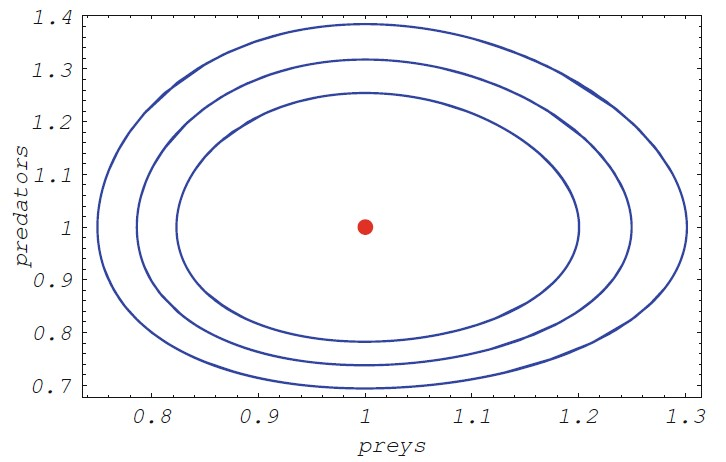
\includegraphics[scale = .5]{Volterra1}
  \end{minipage}
  \ \ \ \ \ \ \ \ \ \ \ \ \ \ \ \
  \begin{minipage}[b]{0.4\textwidth}
    \hspace{-.7cm}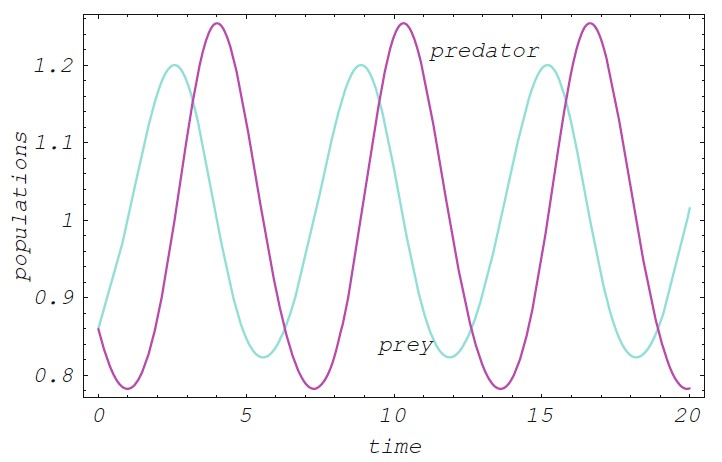
\includegraphics[scale = .5]{Volterra2} 
  \end{minipage}
\end{center}
Questo modello è un ottimo punto di partenza, tuttavia presenta alcune lacune. La lacuna principale è inizialmente si era ipotizzato che la popolazione delle prede crescesse esponenzialmente all'infinito in assenza di predatori, ma questo non è realistico, perchè nessuna popolazione è in grado di sopravvivere con un numero così elevato di individui. \\
Correggiamo il modello supponendo che, in assenza di predatori, la crescita della popolazione delle prede segua un modello logistico, e otteniamo:
\begin{equation}
	\begin{cases}
		\dot{H} = bH\left(1-\frac{H}{K} \right) - sHP \\
		\dot{P} = -dP + esHP
	\end{cases}
\end{equation}
dove $K$ indica la popolazione massima che le prede riescono a sopportare. Per valori alti di $K$, questo modello è solo una perturbazione del modello di Lotka-Volterra. 
\begin{center}
  \begin{minipage}[b]{0.4\textwidth}
    \hspace{.5cm}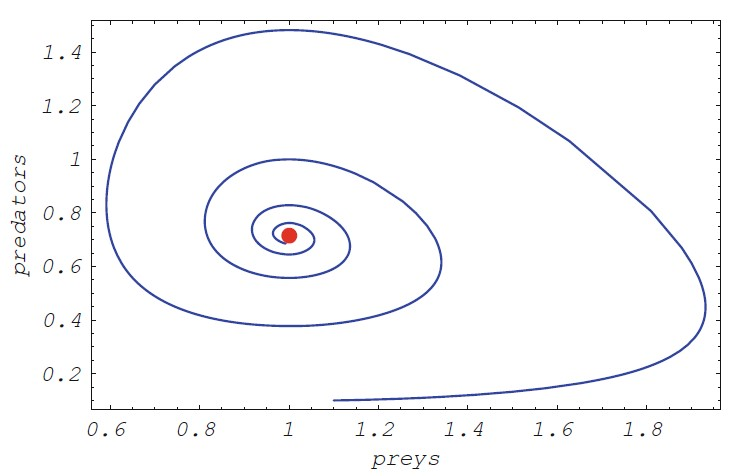
\includegraphics[scale = .5]{Volterra3}
  \end{minipage}
  \ \ \ \ \ \ \ \ \ \ \ \ \ \ \ \ \ \ \
  \begin{minipage}[b]{0.4\textwidth}
    \hspace{-.7cm}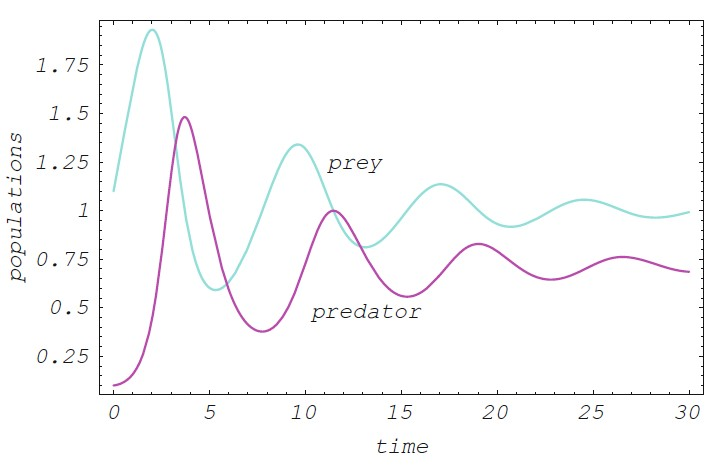
\includegraphics[scale = .5]{Volterra4} 
  \end{minipage}
\end{center}
\subsection{Il caos deterministico}
L'idea del caos deterministico parte dal concetto di sensitività delle condizioni iniziali.  Conoscendo le condizioni iniziali si possono calcolare le evoluzioni, ma cosa succederebbe ad esempio se invece di partire dalle condizioni iniziali $x_0$ partissimo da $x_0 + \delta_0$? Questa domanda è molto importante, perchè avendo un modello è importante capire se un errore nelle condizioni iniziali possa creare un grande errore nell'evoluzione predetta dal modello. Infatti l'errore cresce in maniera esponenziale, perchè l'esponenziale è la funzione che descrive molti fenomeni naturali, quindi avendo un errore iniziale $\delta_0$ questo cresce secondo la legge $\delta (t) = \delta_0 e^{\lambda t}$, dove il coefficiente $\lambda$ si chiama esponente di Ljapourov e da una misura di quanto il sistema è caotico. Possiamo studiare l'importanza di tale coefficiente prendendo il logaritmo dell'equazione precedente:
$$
log \ \delta (t) = log \ \delta_0 + \lambda t
$$
quindi abbiamo un ordine di errore 1 quando: 
\begin{equation}
	t = -\frac{log \ \delta_0}{\lambda}
\end{equation}
Per calcolare $\lambda$ bisogna fare il seguente limite: 
\begin{equation}
	\lambda = \lim_{\delta \rightarrow 0, \ t \rightarrow \infty} \frac{1}{t} log (\phi^t(x+\delta) - \phi^t(x))
\end{equation}
Un processo che si può fare è far crescere un errore per un tempo $\Delta t$, poi fermarla, riscalare e ripartire, e ripetere questo processo pià volte, ottenendo una stima su $\lambda$ secondo la formula: 
\begin{equation}
	\lambda \approx \frac{1}{t} \sum_k log \left(\frac{\delta_k}{\delta_0} \right)
\end{equation}
L'esponente di Ljapounov è una proprietà dell'orbita, non del punto e questo aggiunge complicazione perchè richiede di integrare per un tempo lungo. La nascita del caos richiede di avere un esponente di Ljapounov positivo in un insieme di misura finita. Le orbite devono rimanere limitate. Come è possibile? Supponiamo di prendere un impasto e di stirarlo, in modo da aumentare la distanza, poi lo pieghiamo (a ferro di cavallo), e facendo questo processo a ripetizione le orbite si estendono ma rimangono in un volume finito, e questa è la seconda condizione per avere sistemi caotici. Un altro esempio è una goccia di inchiostro in un bicchiere d'acqua, che si dissolve e sparische. In teoria il sistema potrebbe tornare alla condizione iniziale e la goccia riformarsi, ma la probabilità che ciò accada è molto bassa. E' possibile costruire sistemi caotici? 

\paragraph*{Il gatto di Arnold \\}
Un esempio di sistema caotico è stato fornito da Arnold: La mappa del gatto. \\
\begin{equation}
	\begin{pmatrix}
	x_n \\
	y_n
	\end{pmatrix} = \begin{pmatrix}
	2 & 1 \\
	1 & 1
	\end{pmatrix} \begin{pmatrix}
	x_{n-1} \\
	y_{n-1}
	\end{pmatrix} mod \ 1
\end{equation}
Questa funzione viene definita su un toro, ma la si può immaginare definita su un rettangolo (che piegato nel modo opportuno prende la forma del toro, oppure operando il ragionamento inverso, il rettangolo è il toro tagliato in due direzioni e srotolato), imponendo la condizione che quando una retta esce dal rettangolo, questa faccia il giro e vi rientri dalla parte opposta:
\begin{center}
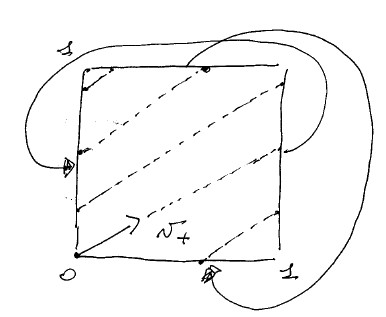
\includegraphics[scale=.8]{Taglio del toro}
\end{center}
La matrice ha determinante uguale a uno, quindi conserva le aree. Si calcolano gli autovalori di tale matrice che risultano $\la_{\pm} = \frac{3+\sqrt{5}}{2}$ (come ci si aspetta dalla conservazione delle aree, il prodotto dei due autovalori è 1). Il primo autovalore $\la_+$ è positivo, quindi esiste una direzione dilatante, ovvero l'autovettore corrispondente a tale autovalore, mentre l'autovettore negativo è legato alla direzione contraente. Tali autospazi sono ortogonali, dal momento che la matrice è simmetrica (per le matrici simmetriche, autovettori legati ad autovalori diversi sono ortogonali). Ora si può osservare il funzionamento di questa mappa. Prendiamo un quadrato (che sarebbe il toro srotolato) e applichiamo la funzione ai 4 vertici. I punti di coordinate $(x,y)$ vengono trasformati in $(2x+y,x+y)$, e questo è l'effetto: 
\begin{center}
  \begin{minipage}[b]{0.4\textwidth}
    \hspace{1cm}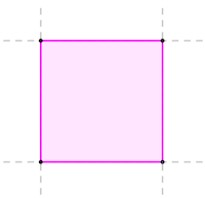
\includegraphics[scale = .8]{Quadrato non trasformato}
  \end{minipage}
  \ \ \ \ \ \ \ \ \ \ \ \ \ \ \ \
  \begin{minipage}[b]{0.4\textwidth}
    \hspace{-2cm}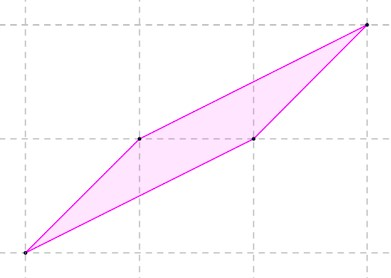
\includegraphics[scale = .8]{Quadrato trasformato} \\
  \end{minipage}
\end{center}
Tuttavia, dal momento che siamo su un toro, quello che esce da destra rientra da sinistra e quello che esce dall'alto rientra dal basso, quindi si riassembla il quadrato iniziale, con dei pezzi che ovviamente non saranno più quelli iniziali, e quindi il quadrato non sarà più quello iniziale. Si nota infatti che il triangolo rosa è l'unico rimasto dentro al quadrato, mentre gli altri sono usciti e rientrati dal lato opposto.
\begin{center}
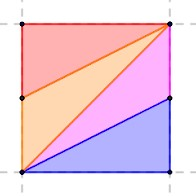
\includegraphics[scale=1.3]{Quadrato riassemblato}
\end{center}
Nella foto sottostante si nota come la foto di un gatto venga tagliata e stracciata, risultando velocemente irriconoscibile, ma essendo il processo deterministico, dopo un certo numero di stadi la foto iniziale dovrà ricomporsi. Si da il caso infatti che la mappa prenda il nome proprio dal fatto che Arnold ne presentò il funzionamento usando la foto di un gatto.
\begin{center}
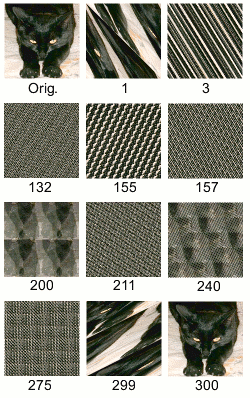
\includegraphics[scale=1]{Arnold_cat}
\end{center} 
Se iteriamo otteniamo un insieme di punti distribuito uniformemente sul piano e si ha l'evoluzione della distribuzione di tali punti, con la condizione della conservazione delle aree: $\int_{T^2} \rho(\vec{r}) dV = 1$ \\ 
L'equazione di continuità dice che il numero di particelle si deve conservare nel processo di applicazione di una trasformazione $T$, per quanto caotico esso sia. La condizione iniziale è $\rho_0(y)dy$, ovvero il numero di particelle nel volume $dy$ e vogliamo arrivare a $\rho(x,n)dx$, ovvero il numero di particelle nel volume $dx$ al tempo n; questo tempo n è discretizzato, quindi equivale a dire dopo n iterazioni, cioè dopo aver applicato la funzione $T$ per n volte. \\ \\
\textbf{DA CORREGGERE!}
 Avendo il numero di particelle nel volume $dx$ al tempo $n$ si può risalive al numero di particelle nel volume iniziale $dy$ al tempo $n=0$ effettuando la trasformazione inversa 
$$
	\rho(x,n) = \rho_0(T^{-n}x)\left|\frac{\partial T^{-n}}{\partial x} \right| 
$$ 
e la derivata è uguale al determinante della matrice, che vale 1 per la conservazione delle aree. Quel fattore va aggiunto proprio per tener conto della conservazione delle aree.\\ A cosa serve questa distribuzione di particelle? \\ \\
Sia $I(x)$ un osservabile del sistema (ovvero una quantità che dipende dall'evoluzione del sistema) , allora il suo valor medio è dato da:
$$
	\lang I \rang (n) = \int I(x) \rho(x,n)dx
$$
Quindi noi siamo interessati alla distribuzione delle particelle perchè ci permette di ricavare i valori di degli osservabili (quindi ne siamo interessati indirettamente). \\
A questo punto ci si chiede se esista una distribuzione $\rho_s$ che rimane invariata nel tempo, ovvero $\rho_s = k$. La risposta è si, e si è osservato che sistemi molto diversi possono avere la stessa distribuzione stazionaria, e questo è collegato al teorema del limite centrale. Se un sistema è in una situazione stazionaria e viene perturbato, poi ritorna alla situazione stazionaria?\\
Sia $\chi_A(x)$ la funzione caratteristica dell'insieme $A$, ovvero la funzione tale che: $
\begin{cases}
1 \ se \ x \in A \\
0 \ se \ x \not\in A
\end{cases}
$ \\
Sia $\rho_0(y) = X_A(y)/m(a)$ e sia $I(y) = X_B(y)$, allora:
$$
	\lang I \rang (n) = \int \chi_B(x) \frac{\chi_A(T^{-n}x)}{m(A)} dx = \int_B \frac{\chi_A(T^{-n}x)}{m(A)}dx = \frac{1}{m(A)} \int_{T^{-n}(B)}\chi_A(y)dy = \frac{1}{m(A)}m(A)m(B)
$$
$$
	m(B) = \int \chi_B(x)\rho_s(x)dx
$$
\textbf{Teorema del ritorno di Poincarrè:} \textit{Un sistema dinamico che conserva i volumi su un compatto torna arbitrariamente vicino alla condizione iniziale.} \\ \\
Tuttavia, questo teorema non dice il tempo necessario per tornare alla condizione iniziale. \\ \\ \\

\textbf{Utilizzo della misura invariante: \\}
Consideriamo il seguente problema. Prendiamo la dinamica creata da $x_n = 2^n$, con $n \geq 1$. Qual è la probabilità di trovare un numero avente 7 come prima cifra? \\
$$
	2^n = (7, . \ . \ .) \ \times 10^k \ \ \ \longrightarrow \ \ \ log_{10} \ 2^n = log_{10} \ (7, . \ . \ .) + k
$$
Quindi possiamo scrivere il il logaritmo di $2^n$ come la somma del logaritmo di un numero avente 7 come prima cifra con un numero intero. Se prendiamo il modulo di 1 di questo numero abbiamo che il modulo di 1 di $k$ è 0, dal momento che questo è un numero intero.
$$
	P(7) \ \ \Longrightarrow \ \ (log_{10} \ 2^n) \ mod \ 1 \in [log_{10}7, log_{10}8]
$$
Quindi abbiamo una dinamica del tipo: $y_{n+1} = (y_n + log_{10} \ 2) \ mod \ 1$ \\
Questa è una dinamica non caotica. Si tratta di una traslazione nell'intervallo $[0,1]$. Questa dinamica non è caotica perchè stiamo semplicemente sommando una quantità finita (non si ha più lo stretching, si ha una traslazione), quindi due punti vicini rimangono vicini. Quindi per questo sistema l'esponente di Ljapounov è nullo. Possiamo calcolare questa probabilità usando il concetto di misura invariante, che in questo caso per $n \rightarrow \infty$ è una distribuzione uniforme nell'intervallo $[0,1]$, e si ottiene:
$$
	P(7) = log_{10}8 - log_{10}7
$$ 

\subsection{Il modello epidemiologico}
Consideriamo uno spazio discretizzato (perchè è più facile da simulare). Un individuo può muoversi in una delle 4 direzioni e queste 4 direzioni sono equiprobabili. Quando la particella arriva al bordo possiamo decidere di far succedere varie cose: \\
1) La particella può muoversi nelle altre 3 direzioni e a ognuna di queste è associata una probabilità del $33 \ \%$. \\ 
2) La particella può muoversi nelle altre 3 direzioni o rimanere ferma dov'è e a ognuna di queste possibilità è associata una probabilità del $25 \ \%$. Questa opzione può portare a un accumulo delle particelle lungo il bordo, quindi bisogna tenere conto di questa cosa. Questo caso e il precedente si chiamano condizioni riflettenti e implicano un'attrattività verso il bordo. \\
3) La particella può muoversi come in tutti gli altri punti della griglia (nelle 4 direzioni e queste sono equiprobabili) e nel caso in cui si muovesse contro il bordo uscirebbe dalla griglia e verrebbe eliminata dalla simulazione. Questa viene chiamata condizione assorbente. \\
4) La particella può muoversi nelle 4 direzioni come nel caso precedente, ma nel caso in cui si muovesse contro il bordo sparirebbe e riapparirebbe dal lato opposto. Questo viene comunemente chiamato effetto pacman.\\
E' chiaro che le condizioni al contorno debbano essere scelte con molta cura, perchè in alcuni casi possono essere determinanti. \\  \\
Per modellizzare l'evoluzione di una pandemia partiamo dividendo la popolazione in 3 gruppi: \\ 
-I suscettibili $S$, ovvero quelli che possono essere infettati. \\ 
-Gli infetti $I$, ovvero gli individui che sono già stati infettati. \\
-I guariti $G$, ovvero gli individui guariti (per scaramanzia prendiamo un'epidemia senza morti). \\ 
Volendo si potrebbe complicare il modello aggiungendo un vaccino e aggiungendo la categoria degli individui vaccinati $V$. 
Possiamo normalizzare queste grandezze, quindi considerare le percentuali sulla popolazione (quindi $S$, $G$ e $I$ sono sempre compresi tra 0 e 1). Quando un individuo infetto incontra un suscettibile, ovvero stanno nella stessa cella, quest'ultimo ha una probabilità $p$ di essere infettato, e questa probabilità rappresenta il parametro di invettività. Gli infetti vanno in quarantena dopo $k$ step temporali e guariscono dopo $m$ step. Definiamo inoltre il parametro di socialità $\beta$ e il tasso di guarigione $\gamma$. Ora possiamo costruire il modello: 
\begin{equation}
\begin{cases}
\dot{S} = -p\beta SI \\
\dot{I} = p\beta SI - \gamma I \\
G = 1 - S - I
\end{cases}
\end{equation}
Si raggiunge l'equilibrio quando $I = 0$ e $S = 1$. Ci si può chiedere se questo punto sia un punto di equilibrio stabile o instabile. Per capire ciò espandiamo rispetto a $I$, che prendiamo piccolo e consideriamo un caso in cui $S \approx 1$ e $I \ll 1$:
$$
	\dot{I} = (p \beta - \gamma)I \ \ \Longrightarrow \ \ I(t) = I_0 \ exp(\la t)
$$
dove si ha $\la = p \beta - \gamma$. Definiamo il fattore $R_t$:
\begin{equation}
	\frac{p\beta}{\gamma}
\end{equation}
Se $\la > 0$ vuol dire che il parametro $R_t > 1$ e questo è il criterio per capire se l'equilibrio è stabile o instabile. \\
Cerchiamo ora un approccio analitico per risolvere il problema:
$$
\frac{d}{dt} log \ S = \frac{\dot{S}}{S} \ \ \longrightarrow \ \ \begin{cases}
\dfrac{d}{dt} log \ S = -p\beta I \\  \\
\dfrac{d}{dt} log \ I = p \beta S - \gamma
\end{cases}
$$ 
Introduciamo le variabili $u = log \ S$ e $v = log \ I$ e le inseriamo nelle equazioni:
$$
\begin{cases}
\dot{u} = -p\beta e^v = -\dfrac{\partial H}{\partial v} \\ \\
\dot{v} = p \beta e^u - \gamma = \dfrac{\partial H}{\partial u}
\end{cases}
$$
Quindi la funzione $H(u,v)$ è un integrale primo del moto per il sistema. Possiamo integrare per ottenerne la formula:
\begin{equation}
	H(u,v) = p \beta (e^u + e^v) - \gamma u
\end{equation}
Si presenta quindi il problema di studiare lo spazio delle fasi $(u,v)$ e quindi le curve di livello di questa hamiltoniana. \\
Facciamo un'ipotesi e supponiamo che $S(0) \approx 1$ e che $0 < I(0) \ll 1$ $\Longrightarrow$ $u(0) \approx 0 \ \ v(0) \approx - \infty$ 
$$
H(S,I) = p \beta (S+I) - \gamma log \ S
 = H_0 > p \beta
$$
Da questo ricaviamo I:
$$
	I = \frac{H_0}{p \beta} - S + \frac{\gamma}{p\beta} log \ S
$$
e consideriamo $I = 0$. Questa situazione si raggiunge quando l'epidemia è nello stato iniziale o quando o quando è finita. Si ottiene quindi:
\begin{equation}
	\boxed{-\frac{\gamma}{p \beta} log \ S = \frac{H_0}{p \beta} - S}
\end{equation}
Graficamente quindi abbiamo una retta con pendenza negativa e una curva logaritmica. Se le due curve non si intersecano la pandemia non parte, mentre studiando l'intersecazione tra le due curve si può trovare $S_{\infty}$, ovvero il numero di suscettibili a fine epidemia (per il covid si è stimato un $S_{\infty}$ del $20 \%$).
\begin{center}
\begin{tikzpicture}
\begin{axis}[
	axis lines = left,
	xlabel = $ S $,
	ylabel = $ Y $,
	xtick = \empty,
	ytick = \empty,
	width = 14cm,
	height = 8cm,
	extra tick style={grid=major, grid style={dotted, cyan}},
	extra x ticks = {0.20318787, 1},
	extra x tick labels = {$S_{\infty}$, $S\frac{H_0}{p \beta}$},
	extra y ticks = {1},
	extra y tick labels = {$S\frac{H_0}{p \beta}$},
]
\addplot[
	domain = 0:1,
	samples = 150,
	color = red,
] {-0.5*ln(x)};
\addplot[
	domain = 0:1,
	samples = 150,
	color = blue,
] {1-x}
node [pos = 0.2, below left] {$Y = \frac{H_0}{p \beta} - S$};

\end{axis}
\end{tikzpicture}
\end{center}
E' interessante anche studiare l'effetto del parametro della socialità sulla pandemia, in particolare sulla durata e il valore massimo degli infetti. In particolare per una pandemia è importante capire come lavorare sul parametro di socialità (chiudendo attività, scuole, lockdown ecc.) senza andare a intaccare troppo sulla popolazione e sull'economia. Per fare ciò è importante avere delle informazioni iniziali e fare un guess, per poterlo poi aggiustare e descrivere al meglio il sistema.

\subsection{Come affrontare un modello microscopico}
I sistemi stocastici come il modello random walk vengono introdotti perchè permettono di trascurare i gradi di libertà nascosti, di considerare il problema solo sotto un aspetto probabilistico e di semplificarlo enormemente. Questo è proprio quello che si fa in meccanica statistica, dove studiare il moto di ogni singola particella sarebbe impossibile e anche non necessario, quindi ci si limita a studiare il sistema nel complesso con concetti statistici. \\ 
In questi modelli si usa spesso l'ipotesi di indipendenza, ovvero si ipotizza la conoscenza di un evento avvenuto nel passato non cambi in alcun modo la probabilità che un evento futuro ha di avvenire (la probabilità condizionata non cambia). \\
Questa ipotesi è ovviamente errata, basti pensare all'effetto farfalla, a molti effetti quantistici come l'entanglement o tutti gli eventi su livello sociale, storico o economico. Tutti questi eventi si basano fortemente sul passato (la seconda guerra mondiale non è scoppiata a caso, e l'invasione della Polonia da parte di Hitler non ha certamente lasciato invariata la probabilità che scoppiasse un nuovo conflitto mondiale). Si usa comunque questa ipotesi, almeno all'inizio, per semplificare i modelli. 
\paragraph{Il legame tra i modelli e il caos \\}
Il legame tra il modello epidemiologico o il random walk e i sistemi caotici sta nel fatto che: Se io faccio muovere una particella nel modello random walk, questa può muoversi in tutto lo spazio, non ci sono vincoli. Questa idea era presente anche nel modello epidemiologico, dove ogni individuo suscettibile poteva incontrare un individuo infetto e infettarsi. Tuttavia, nonostante la particella possa visitare tutto lo spazio, questo non dice nulla sul tempo necessario per fare ciò. In particolare, se ci volesse troppo tempo, la scala di tempo sarebbe troppo lunga anche rispetto a tutta la scala evolutiva del modello. La peste si propagava con la velocità degli iettatori, quindi il modello era dominato dalla mobilità (i modelli attuali infatti devono anche tenere conto della mobilità, i mezzi di trasporto ecc.). L'idea quindi è che il modello raggiunga una distribuzione stazionaria (gli individui sono sparsi in maniera uniforme in tutto lo spazio) e questo permette di calcolare i valori medi degli osservabili, ad esempio il numero degli infetti. Quindi per poter applicare il modello statistico il sistema deve rilassare a una distribuzione costante, come i sistemi caotici, e deve farlo in un tempo breve. Supponiamo di dover tenere sotto controllo l'epidemia a bologna. Il problema è che si potrebbero avere dei percorsi degli individui molto complicati, a causa dei veicoli privati o dei mezzi pubblici (a meno di porre dei vincoli sulla mobilità). Bisogna anche considerare la distanza tra il punto iniziale e il punto finale. Nel modello finale la distanza percorsa sarà sicuramente maggiore della distanza geometrica tra i due punti. 
$$
	E\left(\frac{d(A,B)}{\sqrt{n}}\right) \longrightarrow \sqrt{D}
$$ 
dove $E()$ è la funzione che da il valore di aspettazione (quindi si fa la media), e $D$ prende il nome di coefficiente di diffusione. Chiaramente il coefficiente di diffusione di un'autostrada è molto diverso da quello di una città, perchè l'autostrada è pressocchè dritta, mentre in città ci sono molte curve, incroci e rotonde. Se invece si considerano mobilità non locali (ovvero si possono fare salti nello spazio, ad esempio usando mezzi di trasporto) si parla di diffusioni anomale. 
\paragraph*{Il random walk \\}
Il modello random walk è un modello in cui una particella può muoversi nello spazio in tutte le direzioni (il doppio della dimensione dello spazio considerato) e queste direzioni si considerano tutte equiprobabili.
Consideriamo il random walk unidimensionale. Diciamo che la particella ha una probabilità $p = 1/2$ di muoversi a destra (e una probabilità uguale $q$ di muoversi a sinistra), e diciamo che ogni passo sia lungo $\Delta x$. Quindi il moto della particella si potrebbe immaginare di regolarlo con il lancio di una moneta, ad esempio dicendo che se uscisse testa la particella si muoverebbe a destra, mentre se uscisse croce si muoverebbe a sinistra. In tal caso la dinamica sarebbe:
$$
	T \ \Longrightarrow \ x(t + \Delta t) = x(t) + \Delta x
$$ 
$$
	C \ \Longrightarrow \ x(t - \Delta t) = x(t) - \Delta x
$$
Definiamo quindi una funzione $\xi(t) = \pm 1$ che dipende da cosa esce al tempo $t$, se testa o croce. \\
Allora:
$$
	x(n\Delta t) = x_0 + \sum_k \xi_k \Delta x
$$
dove $\xi_k = \xi(k\Delta t)$. Prendiamo il punto iniziale $x_0 = 0$, quindi il processo è un processo stocastico che dipende dalla realizzazione di $\xi_k$. Possiamo anche calcolare la media e la varianza:
$$
	\lang \xi_k\rang = 0 \ \ \ \ \ \lang \xi_k^2 \rang = 1
$$ 
Gli $\xi_k$ sono eventi indipendendenti, quindi gli eventi sono indipendenti. Questo lo si può verificare facendo:
$$
	\lang \xi_k\xi_h \rang = \lang \xi_k \rang \lang \xi_h \rang = 0 \ \ se \ x \neq h
$$
tuttavia questa è una condizione necessaria ma non sufficiente. 
Possiamo allora applicare il teorema del limite centrale:
$$
	\sum_k \xi_k \Delta x = \sqrt{n\Delta t} \left( \frac{1}{\sqrt{n}} \sum_k \xi_k \right) \frac{\Delta x}{\sqrt{\Delta t}}
$$
e rendendo continua la variabile temporale, $t = n \Delta t$:
$$
	\frac{1}{\sqrt{n}}\sum_k \xi_k \ \longrightarrow \ z(0,1), \ \ \ \ \ z(0,1) \approx \frac{1}{\sqrt{2\pi}} exp\left(-\frac{z^2}{2} \right) 
$$
E a questo punto si può ottenere il coefficiente di diffusione e trovare $x(t)$:
\begin{equation}
	\frac{(\Delta x)^2}{\Delta t} = D \ \longrightarrow \ x(t) = x_0 + \sqrt{Dt}z
\end{equation}
$x(t)$ è una variabile gaussiana con media $x_0$ e varianza $tD$. \\
Ora ci si potrebbe chiedere quale sia la probabilità che la particella esca dal segmento $(-L,L)$ dopo un tempo t. Questa probabilità si trova con:
$$
	1 - \int_{-L}^L \frac{1}{\sqrt{2\pi D t}}exp \left(-\frac{x^2}{2Dt} \right) dx
$$
dove si fa il cambio di variabile e si trova una famiglia di gaussiane in cui cambia la varianza.
\paragraph*{Random walk sul piano \\}
A causa del moto della particella nel piano, $x$ e $y$ sono variabili guassiane e ciascuna di queste segue una gaussiana indipendente, entrambe con la stessa varianza perchè supponiamo che le direzioni siano indipendenti, quindi il moto complessivo è il prodotto delle gaussiane:
\begin{equation}
	(x,y) \approx \frac{1}{2\pi Dt}exp\left(-\frac{(x^2+y^2)}{2Dt}\right) = \rho(x,y,t)
\end{equation}
e possiamo definire il coefficiente di diffusione come: $D = \frac{\Delta x^2}{\Delta t} = \frac{\Delta y^2}{\Delta t}$. \\
Il random walk nasce dalla distribuzione binomiale, ma grazie alla possibilità di applicare il teorema del limite centrale possiamo studiarlo con una distribuzione gaussiana, di cui possiamo studiare il valor medio e la varianza. 
\begin{center}
  \begin{minipage}[b]{0.4\textwidth}
    \hspace{0cm}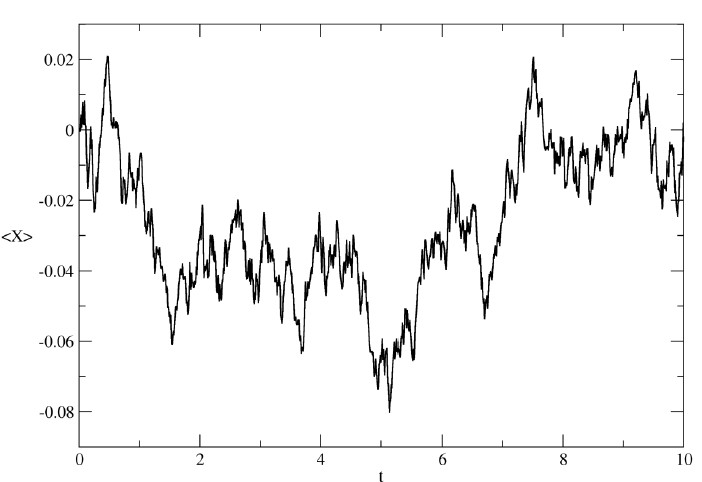
\includegraphics[scale=.55]{Media random walk}
  \end{minipage}
  \ \ \ \ \ \ \ \ \ \ \ \ \ \ \ \ \ \ \ 
  \begin{minipage}[b]{0.4\textwidth}
    \hspace{-1cm}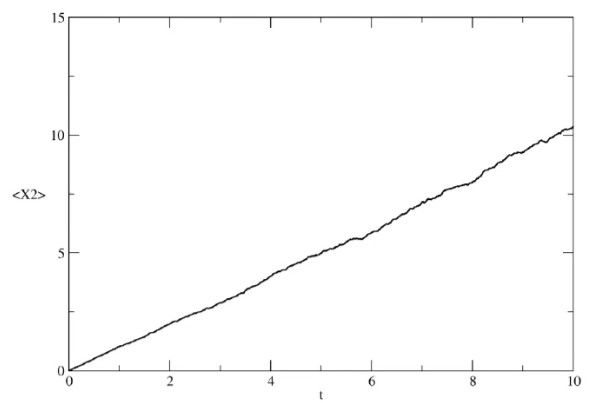
\includegraphics[scale=.65]{Varianza random walk} 
  \end{minipage}
\end{center}
Se osserviamo la varianza, che cresce linearmente nel tempo con coefficiente angolare uquale alla diffusione, si trova che un processo che sembra molto fluttuante guardando la media (che oscilla) risulta stabile quando si osserva la varianza. Questo è dovuto al fatto che, se i valori statistici che fluttuano sono piccoli, come nel caso del random walk, gli effetti di fluttuazione possono sembrare più grandi di quanto non siano. \\ \\
Nel grafico sotto si nota come cambia il random walk quando cambia il passo ad ogni istante temporale. Nella linea blu, quella con il passo più corto, la traiettoria va a riempire maggiormente lo spazio.
\begin{center}
	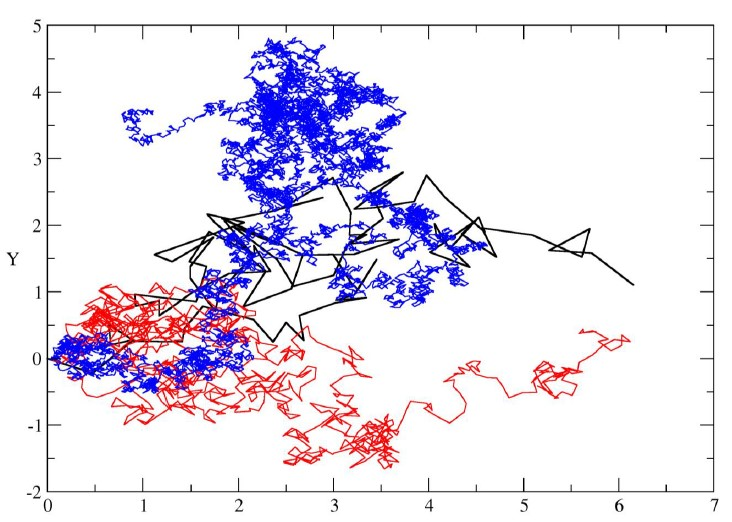
\includegraphics[scale=.7]{Random walk 2D}
\end{center}
Se vogliamo calcolare la distanza radiale percorsa dobbiamo fare un cambio di variabile: 
$$
\begin{cases}
	x = r cos \theta \\
	y = r sin \theta
\end{cases} \ \ \longrightarrow \ \ \rho(x,y,t)dxdy = \frac{1}{2 \pi D t} exp(-\frac{r^2}{2Dt}) r dr d\theta
$$
Dove si integra in $\theta$: 
$$
	\frac{r}{Dt} exp(-\frac{r^2}{2Dt}) = \rho(r,t)
$$
dove $r$ è positivo. \\
E si può a questo punto trovare il valore medio della distanza radiale: 
\begin{equation}
	\lang r \rang = \int_0^\infty \frac{r^2}{Dt} exp \left(-\frac{r^2}{2Dt} \right)dr = \sqrt{\frac{\pi Dt}{2}}
\end{equation}
E si ha che $\lang r \rang \propto \sqrt{Dt}$.
\begin{center}
	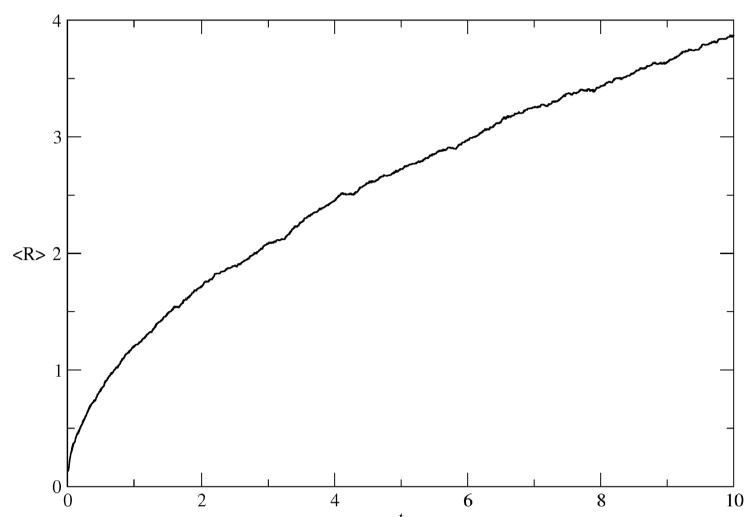
\includegraphics[scale=.7]{Distanza radiale media RW}
\end{center} 
\paragraph*{Modellino economico \\}
Abbiamo una griglia e $M$ individui che si possono muovere dentro essa. Questi individui, indicizzati da un indice $k$, hanno una quantita $n_k$ che rappresenta i loro soldi. Quando due individui si incontrano, si lancia una moneta e ogni idividuo ha una probabilità di $1/2$ di perdere o di guadagnare soldi dall'altro individuo. In questo processo si ha quindi un vincolo che è la conservazione della capitale totale del sistema:
\begin{equation}
	\sum_{k=1}^M n_k = N \ \ \ con \ n_k \geq 0
\end{equation}
Questo vincolo impone che gli individui non possano indebitarsi. \\
Durante la simulazione può succedere che degli individui diventino poveri, ovvero perdano tutti i soldi. In questo caso bisogna decidere quale condizione al contorno si vuole applicare: \\
1) Si può decidere di non giocare con l'individuo senza soldi, perchè l'individuo con i soldi non ha possibilità di guadagno. In questo scenario un individuo che diventa povero rimane povero per sempre. \\
2) Si gioca anche con gli individui poveri nonostante gli individui con i soldi non abbiano margine di guadagno, e nel caso in cui il povero perda non succede nulla, mentre nel caso in cui il ricco perda, il povero riguadagna qualcosa (per il povero questa è quella che si chiama win-win). \\ \\
Questo tipo di sistema, che è un sistema statistico, si dice microcanonico (usando la terminologia della meccanica statistica) perchè i soldi, che fanno la parte dell'energia, possono essere scambiati tra i sistemi ma non possono essere scambiati con l'esterno, perchè il capitale totale deve essere conservato. Ci si può chiedere ora se il sistema tende a un qualche tipo di equilibrio e che forma abbia questo equilibrio, ovvero se la ricchezza si distribuisce uniformemente o se si formano degli addensamenti di ricchezza. \\
Vogliamo quindi calcolare in quanti modi diversi le monete possono essere distribuite tra gli $M$ individui, ovvero vogliamo calcolare tutte le combinazioni possibili. Stiamo quindi supponendo che tutte le possibili distribuzioni di ricchezza siano equiprobabili. E' ragionevole fare questa scelta quando non abbiamo motivo di pensare che ci sia un bias. Questo si fa con il coefficiente binomiale:
\begin{equation}
	\Omega = \begin{pmatrix}
	M + N - 1 \\
	N-1
	\end{pmatrix} = \frac{(M+N-1)!}{(N-1)!M!}
\end{equation}
Questo vuol dire che se lascio che il sistema vada all'equilibrio, posso osservare uno qualsiasi di questi stati, ognuno dei quali ha una probabilità $p = 1/\Omega$. \\
Tutti gli individui sono uguali, quindi diciamo che ogni particella è rappresentativa della popolazione (non ci sono individui più fortunati e altri più sfortunati). Ci si chiede ora quale sia la probabilità $p(n)$ che un certo individuo abbia una certa quantità $n$ di monete. Questa probabilità è data dal modo in cui possiamo distribuire tutte le monete su tutti gli individui:
\begin{equation}
	p(n) = \frac{\begin{pmatrix}
	M+N-2-n \\
	M-2
	\end{pmatrix}}{\begin{pmatrix}
	M+N-1 \\
	M-1
	\end{pmatrix}} \ \ \longrightarrow \ \ \lim_{M\rightarrow \infty} \frac{M}{N} \left(1 - \frac{n}{N} \right) \ \rightarrow \ \underline{\frac{1}{\overline{n}}exp(-n/\overline{n})}
\end{equation}
dove $\overline{n} = N/M$. \\
Quindi quello che si ottiene è una distribuzione esponenziale, e non una gaussiana. Questo vuol dire che anche in un sistema perfettamente giusto (come questo ipotizzato qui, in cui non ci sono bias, non si possono fare debiti e anche i poveri possono riguadagnare ricchezza) si ha un  numero elevato di poveri e un numero molto limitato di ricchi. \\
Questa distribuzione ricorda molto la distribuzione dell'energia di Maxwell-Boltzmann che si trova in meccanica statistica:
\begin{equation}
	\frac{1}{T}exp \left(-\frac{E_n}{T} \right)
\end{equation}
con $E_n = n \Delta E$ \\ \\
In realtà la distribuzione della ricchezza in un modello reale segue una distribuzione a potenza.
\begin{center}
	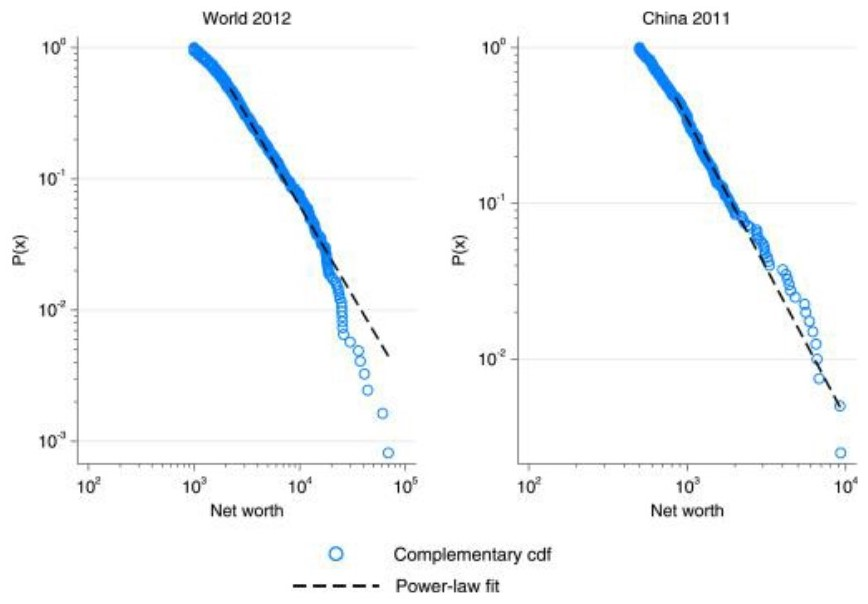
\includegraphics[scale=.65]{Income distribution}
\end{center}
Dobbiamo quindi correggere il modello economico, e in particolare dobbiamo correggere il modo in cui avvengono gli scambi di denaro. \\
Supponiamo che la probabilità che un individuo ha di guadagnare o perdere denaro non sia più costante, bensì dipenda dal suo capitale, ovvero che sia una funzione $\pi_{\pm}(n)$. \\
La probabilità che una persona cambi il proprio capitale deve essere uguale alla probabilità che un individuo con più soldi ne perda e uno con meno soldi ne guadagni:
\begin{equation}
	\pi_+(n-1)p(n-1) = \pi_-(n+1)p(n+1) = \pi_+ (n)p(n)+ \pi_-(n)p(n)
\end{equation}
Si può fare anche il bilancio tra due singoli individui, ovvero un bilancio locale (o bilancio dettagliato):
\begin{equation}
	\pi_+(n-1)p(n-1) - \pi_-(n)p(n) = 0
\end{equation}
Ora ipotizziamo che $\pi_-(n)-\pi_+(n) = a$ e che $\frac{1}{2}(\pi_+(n)+\pi_-(n)) = bn$, ovvero ipotizziamo che avendo più denaro, al probabilità di acquisirne dell'altro è più grande della probabilità di perderne. Per essere precisi bisognerebbe considerare non il capitale del singolo individuo considerato, bensì la differenza di capitale tra i due individui. \\
Ora facciamo uno sviluppo in Taylor della formula 29 otteniamo la seguente equazione differenziale in funzione di $p(n)$:
$$
	ap(n)+\frac{\partial}{\partial n}(bn)p(n) = 0 \ \ \longrightarrow \ \  -\frac{a}{bn} = \frac{1}{(bn)p(n)}\frac{\partial}{\partial n}(bn)p(n)
$$
$$
	\Longrightarrow \ -\frac{a}{b}log(n) = log\left((bn)p(n)\right) + cost
$$
Si ottiene quindi:
\begin{equation}
	p(n) \propto \frac{1}{bn} \cdot \frac{1}{n^{a/b}} = \frac{A}{n^{a/b+1}}
\end{equation}
Questa si chiama "preferential attachment", ovvero più si ha, più è alta la probabilità di guadagnare e questo è proprio il tipo di dinamica che può generare una legge a potenza. 
Usando il bilancio dettagliato si trova che:
$$
	p(n) = \frac{\pi_+(n-1)}{\pi_-(n)}p(n-1)
$$
questa è una relazione ricorsiva, che può quindi essere reiterata:
$$
	p(n) = \prod_{k=1}^n \frac{\pi_+(k-1)}{\pi_-(k)}p(0)
$$
dove $p(0)$ normalizza la distribuzione. \\
Dal bilancio dettaglaito:
$$
	\pi_+(n-1/2)p(n-1/2) - \pi_-(n+1/2)p(n+1/2) = 0
$$
Ora possiamo sviluppare in approssimazione di piccoli cambiamenti di capitale:
$$
	(\pi_+(n)+\pi_-(n))p(n) - \frac{1}{2}\frac{\partial}{\partial n} (\pi_+(n)+\pi_-(n))p(n) \approx 0
$$
da cui:
$$
	a p(n) + \frac{\partial}{\partial n}(bn)p(n) \approx 0
$$
Ponendo $\pi_+(n) \approx bn - a/2$, $\pi_-(n) ) bn + a/2$, per $n \gg 1$ si ha:
$$
	p(n) - p(n-1) ) \left( \frac{bn-a/2}{bn + a/2}-1\right)
$$
questa relazione la possiamo approssimare con una derivata:
$$
	\frac{dp}{dn} = -\frac{a}{bn}p(n-1) \ \ \Longrightarrow \ \ n^{-a/b} \approx \ p(n)
$$
per n grandi.
\subsection{Ranking distribution} 
Un ranking è un insieme di misure di una stessa grandezza tra le quali esiste una relazione d'ordine. Riducendo misure dettagliate a una sequenza di numeri ordinati, i ranking rendono possibile ottenere informazioni complesse seguendo specifici criteri. Un esempio di utilizzo dei ranking si ha nelle pagine web, dove il motore di ricerca mostra all'utente i risultati della sua ricerca in un ordine dettato dalla stima della loro rilevanza, in modo da permettergli di trovare velocemente l'informazione di cui necessita. In questo caso la grandezza è la rilevanza del risultato alla ricerca.
Un altro esempio di ranking si ha nella sottostante, che mostra il ranking della popolisità (quindi la grandezza misurata è la popolazione della città) di 300 città europee. La scala è log-log, quindi dal momento che il grafico è una retta ne deriva che il ranking segue una distribuzione a potenza. Questo si può spiegare con il fatto che storicamente, quando la popolazione è stabile, questa tende a migrare verso le città per via delle maggiori opportunità. Le grandi città hanno quindi un preferential attachment. 
\begin{center}
	\includegraphics[scale=.75]{Ranking città}
\end{center}
Sia $x$ una variabile aleatoria e siano $\{x_1, . . . , x_N \}$ un sample di osservazioni sperimentali ordinate, ovvero tali che $x_1 \geq x_2 \geq . \ . \ . \ \geq x_N$. La distribuzione del ranking è creata assegnando alla posizione $j$ dell'ordinamento il suo valore del sample, ed è data da $x_j = f(j)$, e usualmente si normalizza con $x_j/x_1 = y_1$. \\
Per definizione $j/N$ è la frequenza dell'evento $\{x \ | \ x \geq x_j\}$, ovvero è la probabilità che la grandezza $x$ abbia valori più grandi di $x_j$ per valori maggiori di $j$. La distribuzione cumulata è invece definita definita come $F(x) = P\{u \ | \ u \leq x_j\}$, ovvero la probabilità che il valore $u$ sia più piccolo del valore $x$, e come è noto, questa probabilità è uguale all'integrale della distrubuzione da $-\infty$ a $x$. La relazione tra la frequenza $j/N$ e la distribuzione cumulata è data da:
$$
	F(x_j) = 1 - \frac{j}{N} = 1 - \frac{J(x_j)}{N}
$$
dove $J(x_j)$ è l'inverso del ranking, ovvero la funzione che restituisce la posizione di un certo valore di $x$ nell'ordinamento del sample. \\
Essendo la probabilità cumulata l'integrale della distribuzione di probabilità, la sua derivata dà proprio la distribuzione:
$$
	p(x) = \frac{dF}{dx} \ \ \longrightarrow \ \ p(x) = -\frac{1}{N} \frac{dJ}{dx}
$$
Ad esempio, possiamo considerare la sequente funzione di frequenza: 
$$
	f(j) = \dfrac{x_1}{j^a} \ \rightarrow \ J(x_j) = \left(\dfrac{x_j}{x_1}\right)^{-\frac{1}{a}}
$$
e ottenuta l'inversa del ranking si può trovare la distribuzione di probabilità:
$$
	p(x) = \frac{1}{aM}\left(\frac{x}{x_1}\right)^{-\frac{1}{a}-1} \propto \ \frac{1}{x^b}
$$
che è quindi una distribuzione a potenza per valori $b>1$.
\subsection{Il giocatore rovinato}
Un giocatore d'azzardo in un casinò ha un capitale $k$, compreso tra $0$ e $N$, e gioca con una probabilità $p$ di vincere e $q = 1 - p$ di perdere. Diciamo quindi che se arriviamo a $k=N$ abbiamo vinto, mentre se arriviamo a $k=0$ usciamo dal gioco e abbiamo perso, perchè non abbiamo più capitale da scommettere. E' quindi un modello che simula un giocatore in un casinò. Possiamo trattare questo modello in maniera simile al random walk. \\
Sia $P_N(k)$ la probabilità di vincere le $N$ monete avendo un capitale iniziale $k$. Questa probabilità la si può valutare studiando gli scambi tra stati vicini:
$$
	P_N(k) = pP_N(k+1) + q P_N(k-1)
$$
dove le condizioni al contorno sono $P_N(0) = 0$ e $P_N(N) = 1$, e in più abbiamo supposto che ci sia indipendenza dal passato, ovvero che la probabilità di vincere di vincere uno step sia invariante dal fatto di aver vinto o perso lo step precedente. Quindi noi schematizziamo il problema dicendo che la probabilità di vincere il gioco partendo da $k$ monete è la probabilità di vincere avendo perso una volta, e quindi partendo da $k-1$ monete, sommata alla probabilità di vincere dopo aver vinto uno step, e quindi partendo da $k+1$ monete. \\
Riscriviamo la probabilità nel modo seguente:
$$
	P_N(k+1) - P_N(k) = \frac{q}{p} (P_N(k) - P_N(k-1))
$$
questa è una equazione ricorsiva e può essere reiterata: $ P_N(k+1) - P_N(k) = \left(\dfrac{q}{p} \right)^k P_n(1) $
$$
	  \longrightarrow \ \ \sum_{k=1}^{i-1}(P_N(k+1)-P_N(k)) = P_N(i)-P_N(1) = \sum_{k=1}^{i-1} \frac{q}{p} (P_N(k) - P_N(k-1))
$$
si ottiene quindi:
$$
	P_N(i) = \frac{1-\left(\dfrac{q}{p} \right)^i}{1-\left(\dfrac{q}{p}\right)}P_N(1) \ \ \longrightarrow \ \ P_N(1) = \frac{1-\left(\dfrac{q}{p}\right)}{1-\left(\dfrac{q}{p}\right)^N} \ \ 
	\longrightarrow \ \ P_N(k) = \frac{1-\left(\dfrac{q}{p}\right)^k}{1-\left(\dfrac{q}{p}\right)^N}
$$
dove abbiamo usato la condizione al contorno che $P_N(N) = 1$. \\
Consideriamo il caso limite in cui la probabilità di vincere è maggiore di quella di perdere. Allora se $N \rightarrow \infty$ si ha $P_\infty (k) = 1 - \left(\dfrac{q}{p} \right)^k$. \\
E da questo risulta che la probabilità di essere rovinato è:
\begin{equation}
	1-P_\infty (k) =  \left(\frac{q}{p} \right)^k
\end{equation}
e notiamo che questa probabilità tende a 0 quando abbiamo un capitale di partenza che va a infinito. \\
Se ora consideriamo che $p=q=0.5$ si ha:
\begin{equation}
	P_n(k) = \frac{k}{N} \ \ \ 1-P_n(k) = 1 - \frac{k}{N}
\end{equation}
questo vuol dire che anche se il gioco in un casinò fosse perfettamente corretto e onesto, si avrebbe comunque una probabilità molto alta di essere rovinati. Questo è dovuto al fatto che un giocatore punta a guadagnare il più possibile e quindi continua a giocare, ma il banco non si rovinerà mai, perchè ha un capitale massimo enorme, mentre il giocatore ha un capitale massimo significativamente più basso, e quindi una probabilità molto più alta di finire rovinato.

\subsection{Entropia e informazione}
Sia $x$ una variabile random a valori discreti uguali alle lettere dell'alfabeto. I valori di questa variabile, ovvero i caratteri, possono combinarsi per formare delle sequenza, dove la realizzazione di ogni carattere è indipendente:
$$
	\{x_k\}_{k=1}^N = A, B, C, A, ...
$$
e visto che le realizzazioni sono indipendenti,la sequenza ha una probabilità: $P(\{x_k\})=p(x_1)...p(x_k)$ \\
Possiamo immaginare anche una proteina in questo modo, come una sequenza di amminoacidi, anche se questo è impreciso perchè le proteine si formano secondo dei meccanismi biologici ben precisi e non a random. \\
Possiamo anche fare un coding di questo tipo per caratterizzare la mobilità di un individuo, ad esempio controllandone la posizione ogni ora e assegnando una lettera a ogni posizione. Un altro modo per codificare la mobilità consiste invece nel contare il numero di visite in ogni luogo. Possiamo ad esempio codificare la traiettoria nella mappa del gatto, dividendo il quadrato in 4 quadranti e assegnare a ogni quadrante una lettera. \\
Anche quando parliamo codifichiamo un pensiero, ovvero trasmettiamo un'informazione tramite una sequenza di simboli che vengono poi interpretati per ottenere questa informazione. \\
Defininiamo l'informazione portata da un carattere (o da una sequenza di caratteri), ad esempio A, come il logaritmo della sua probabilità.
Definiamo ora l'entropia di Shannon:
\begin{equation}
	S = -\sum_k P(x_k)log P(x_k)
\end{equation}
L'idea di questa entropia è che un evento molto probabile trasporti poca informazione. \\
Se consideriamo ora una coppia di caratteri indipendenti
$$
	P(\{x_{k_1}, x_{k_2}\}) = P(x_{k_1})P(x_{k_2})
$$
e avendo questa probabilità possiamo studiare l'entropia della coppia di caratteri:
$$
	S = -\sum_{k_j} P(\{x_{k_1}, x_{k_2}\})log P(\{x_{k_1}, x_{k_2}\}) = P(x_{k_1})P(x_{k_2}) log P(\{x_{k_1}, x_{k_2}\}) = P(x_{k_1})P(x_{k_2}) 
$$
$$
	= S_1 + S_2
$$
quindi l'entropia di Shannon di una coppia di eventi è la somma delle entropie dei singoli eventi. \\
La misura di Shannon rappresenta il numero ottimale di bit necessari per memorizzare la sequenza. Notiamo quindi che l'entropia e l'informazione sono una cosa diversa: La sequenza "semprecaromifuquest'ermocolle" ha entropia minore di "actraxax", ma la prima trasporta molta più informazione. \\
Se a una sequenza $\{x_1,x_2,...\}$ aggiungiamo un carattere, l'entropia di Shannon misura un aumento di informazione.
Consideriamo ora la collerazione tra i caratteri:
$$
	P(\{AB\}) = P(B|A)p(A)
$$
se questa probabilità è diversa dal prodotto delle singole probabilità vuol dire che i caratteri non sono indipendenti, quindi si ha una correlazione. \\
La legge dei grandi numeri implica che data una sequenza di caratteri $\{x_k\}$, la probabilità di ottenere un certo carattere (ad esempio $A$) è:
$$
	P(A) = \lim_{N\rightarrow \infty} \frac{N^o\{x_j = A\}}{N}
$$
se è presente un correlazione $P(A)$, questo non cambia la probabilità di uscita di un singolo simbolo. 
$$
	P(AB) = \frac{N^o\{x_ix_j = AB\}}{N-1}
$$
La probabilità condizionata $P(B|A)$ definisce una matrice di transizione: $P_{ij} = P(x_j|x_i)$ \\
dove $i$ si riferisce all'evento precedente e $j$ si riferisce a quello successivo. \\
Tale matrice deve avere certe caratteristiche: \\
-Per ogni coppia di indici, gli elementi della matrice devono essere compresi tra 0 e 1, perchè sono probabilità. \\
-La somma degli elementi della matrice deve dare $1$. \\
Se queste condizioni sono rispettate, $P_{ij}$ si dice matrice stocastica. \\
Supponiamo di conoscere la probabilità $P_i$ di avere un carattere $x_i$, qual è allora la probabilità di ottenere il carattere $x_j$ al passo successivo? \\
$$
	P^{n+1}_j = \sum_iP_{ij}P^n_i 
$$
Esiste una $P^s_i$ tale che:
$$
	P^s_j = \sum_i P_{ij}P^s_i
$$
ovvero un autovettore con autovalore unitario. \\
Sia $\vec{1} = (1,...,1)$. Allora questo vettore è un autovettore con autovalore unitario per $P_{ij}$, ma allora anche la trasposta ha autovalore unitario, quindi esiste un autovettore $P_i^s$ unitario. \\
Dal momento che tutti gli elementi della matrice sono positivi, anche gli elementi del vettore unitario devono essere positivi, e possiamo normalizzarlo in modo che la somma dei suoi elementi dia 1. \\
Sia $\vv$ tale che la somma dei suoi elementi è nulla (iperpiano). Allora $v'_j = \sum_i P_{ij}v_i$ ha la stessa proprietà, quindi questo iperpiano è invariante. \\
Da questo segue che:
$$
	se \ \sum_iP_i = 1 \ \ \Longrightarrow \ \ \sum_j P^{n+1}_j = \sum_{ij} P_{ij} P_i^n = 1
$$ 	
A questo punto ci chiediamo, se abbiamo una sequenza di simboli, e aggiungiamo un simbolo, quanta informazione abbiamo aggiunto?
$$
	P(\{x_1,...,x_{n+1}\}) = P(x_{n+1}|x_n)P(\{x_1,...,x_n\})
$$
Calcoliamo l'entropia della posizione $n+1$:
$$
	S_{n+1} = - \sum P(\{x_1,...,x_{n+1}\}) log  P(\{x_1,...,x_{n+1}\}) = 
$$
$$
	- \sum P(x_{n+1}|x_n)P(\{x_1,...,x_n\}) \left[log P(x_{n+1}|x_n) + log P(\{x_1,...,x_n\}) \right] = 
$$
$$
	-\sum^n P(\{x_1,...,x_n\}) log P(\{x_1,...,x_n\}) - \sum_{ij} P_j^sP(x_i|x_j)logP(x_i|x_j)
$$
Quindi si ottiene:
\begin{equation}
	S_{n+1} = S_n - \sum_{ij} P_j^sP_{ij}logP_{ij}
\end{equation}
\subsection{Effetto di memoria: Il modello broken stick}
Cerchiamo ora di capire il collegamento tra gli effetti di memoria e le distribuzioni. \\
Immaginiamo di avere un segmento di lunghezza unitaria, e inseriamo un punto $x_1$ in una posizione casuale. Questo inserimento impedisce che un altro punto venga inserito nel pezzo $[0,x_1]$, quindi è come se tagliassimo questo pezzo dal segmento.  \\
A questo punto possiamo prendere il segmento rimanente e fare un altro inserimento e ritagliarlo, e così via. Il processo viene iterato, ma chiaramente ha una memoria di tutto, perchè la lunghezza del segmento dopo un certo numero di iterazioni dipende da tutte le iterazioni precedenti. \\
Ci chiediamo ora quale sia la distribuzione dei segmenti ottenuti. \\
L'idea alla base è che nel passaggio dal segmento iniziale al successivo si abbia un riscalamento, perchè il modo in cui inserisco i punti è sempre lo stesso, ma sto riscalando l'intervallo spaziale in cui questi punti possono essere inseriti. Si può capire facilmente questo concetto prendendo il segmento accorciato dopo la prima iterazione, e immaginare di riscalare la scala di lunghezza; con l'opportuno riscalamento potremmo misurare una lunghezza del bastone uguale a quella iniziale. \\
Il punto in cui tagliamo il segmento viene inserito in modo casuale secondo una distribuzione uniforme tra $0$ e $1$, che ha media $1/2$, percui mediamente il segmento verrà diviso a metà:
$$
	\lang x \rang = \frac{1}{2}, \ se \ x \in [0,1]
$$
dobbiamo quindi avere un'invarianza di scala per il riscalamento $y \rightarrow y/2. $\\
Per quanto detto, la distribuzione dei due segmenti dopo $M+1$ iterazioni deve essere simile alla distribuzione dopo $M$ partendo da un segmento lungo $1/2$, purchè $M$ sia grande. \\
Per $M \gg 1$:
$$
	\rho_{M+1}\left(\frac{y}{2}\right)\frac{dy}{2} = \rho_{M}(y)dy
$$
cerchiamo quindi una distribuzione del tipo: $\rho(y/2) = 2 \rho(y) \ \longrightarrow \ \rho(y)\approx 1/y$. \\
Questo tipo di processo si dice "a memoria assoluta", perchè il pezzo di segmento tagliato viene elimitano dopo ogni iterazione, e non è più accessibile o modificabile. Questo tipo di comportamento si ritroma in molti processi biologici, dove ad esempio, dopo aver silenziato una sequenza di DNA questa non si può de-silenziare.
A questo punto possiamo modificare il processo, aggiungendo a iterazione la possibilità di tagliare il segmento, con probabilità $p$ o di lasciarlo com'era prima dell'iterazione, con probabilità $1-p$, e in questo caso si otterrebbe una legge a potenza.
\subsection{Modelli a memoria finita: I modelli di Markov}
Un tipo particolare di modelli a memoria sono i modelli di Markov. Questi sono modelli a memoria finita, in cui la probabilità di un sistema di passare in un certo stato dipende solo dallo stato immediatamente precedente, ma non da come il sistema è arrivato in quello stato. \\
La condizione matematica dei processi markoviani è, per una grandezza generica $X$ dipendente dal tempo:
\begin{equation}
	P(X(t_{n+1})=x_{n+1}|X(t_n)=x_n, ..., X(t_0)=X_0) = P(X(t_{n+1})=x_{n+1}|X(t_n)=x_n)
\end{equation}
Capiamo quindi che il modello broken-stick è un processo assolutamente non markoviano, perchè ha memoria infinita. \\
Condideriamo ora un esempio di modello markoviano:\\
Abbiamo un insieme finito di stati rappresentati da dei caratteri, e possiamo avere delle transizioni tra questi caratteri.
\begin{center}
	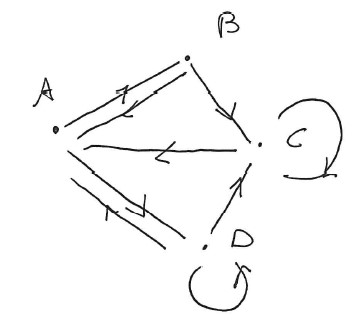
\includegraphics[scale=.85]{Grafo processo non markoviano}
\end{center}
Ogni link direzionale rappresenta una possibile transizione con peso $\pi_{ij}$, dove questa ordinazione degli indici indica una transizione dallo stato $j$ allo stato $i$. Ogni link rappresenta sia la possibilità di passare da un simbolo all'altro, sia il peso di tale transizione. Questo genera quindi un grafo, o network. Le transizioni tra i vari caratteri possono essere espressi tramite un coding, rappresentando quello che si chiama random walk su grafo. \\
Consideriamo il caso in cui abbiamo 3 simboli, $\{A,B,C\}$, a cui assegnamo rispettivamente gli indici $(1,2,3)$, e la matrice di transizione:
$$
	\pi_{ij} = \begin{pmatrix}
	0 & 1/2 & 1/2 \\
	1/2 & 0 & 1/2 \\
	1/2 & 1/2 & 0
	\end{pmatrix}
$$
dove abbiamo trascurato i "self-loop", come si può notare dagli elementi della diagonale nulli. \\
Questa matrice si dice stocastica, ovvero una matrice che ha somma degli elementi delle righe (o delle colonne) uguale a $1$. Questa matrice in particolare è bistocastica, perchè è stocastica sia rispetto alle righe che rispetto alle colonne. \\
Facendo i calcoli si vede che gli autovalori di questa matrice sono $1$, $-1/2$ e $-1/2$.
In questo caso tutti i link pesano $1/2$, e si ottiene quindi il seguente grafo:
\begin{center}
	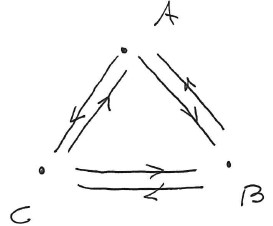
\includegraphics[scale=.9]{Grafo equiprobabile}
\end{center}
Data una probabilità iniziale $p_j^o$ abbiamo l'evoluzione:
$$
	p_j^{n+1} = \sum_j \pi_{ij} p_j^n \ \ \Longrightarrow \ \ \lim_{n \rightarrow \infty} P^n = \left(\frac{1}{3},\frac{1}{3},\frac{1}{3}\right)
$$
Prendiamo ora la seguente matrice:
$$
	\pi_{ij} = \begin{pmatrix}
	0 & 1/3 & 2/3 \\
	2/3 & 0 & 1/3 \\
	1/3 & 2/3 & 0
	\end{pmatrix}
$$
In questo caso le transizioni non sono più equiprobabili, bensì il moto più probabile è quello lungo un loop.
\begin{center}
	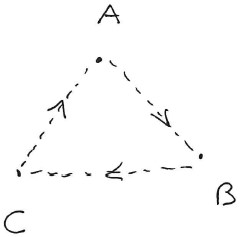
\includegraphics[scale=1]{Grafo loop}
\end{center}
Vediamo quindi che se abbiamo il simbolo A, è più facile che questo passi allo stato B, piuttosto che allo stato C. \\
Se studiamo ora la distribuzione stazionaria, notiamo che questa è la stessa del caso precedente: 
$$
	P^s = \left(\frac{1}{3},\frac{1}{3},\frac{1}{3}\right)
$$ 
La differenza principale tra le due transizioni che abbiamo considerato si può vedere considerando le sequenze e leggendole al contrario. Nel primo caso le sequenze invertite hanno la stessa probabilità di quelle dritte, e il processo si dice reversibile. Nel secondo caso invece le sequenze invertite proseguono in modo contrario alle sequenze dritte (perchè queste seguono un loop, quindi leggendole al contrario ottengo un loop nel senso opposto), quindi non si ha reversibilità. Capiamo quindi che la differenza principale tra questi processi è la perdita della reversibilità. \\
La perdità della reversibilità stà nello studio del bilancio dettagliato che abbiamo visto nelle sezioni precedenti. 
$$
	\pi_{ij}P_j^s = \pi_{ji}P_i^s \ \ \longrightarrow \ \ 1) \ \pi_{13}p_3^s = \frac{1}{2}\cdot\frac{1}{3} = \pi_{31}p_1^s
$$
$$
	\ \ \ \ \ \ \ \ \ \ \ \ \ \ \ \ \ \ \ \ \ \ \ \ \ \ \ \ \ \ \  \longrightarrow \ \ 2) \ \pi_{13}p_3^s = \frac{2}{3}\cdot\frac{1}{3} \neq \frac{1}{3}\cdot\frac{1}{3} = \pi_{31}p_1^s
$$
Nel primo caso si ha un bilancio tra il numero di transioni da A a B e di quelle da B ad A, mentre nel secondo tipo di transizione non si ha questo bilancio dettagliato, si può avere solo un bilancio globale, ma è proprio il bilancio dettagliato quello che garantisce la reversibilità, e questo è il motivo per cui il secondo processo risulta irreversibile.
\paragraph*{Giochi di Penney \\}
Consideriamo ora un gioco interessante che applica il concettro di grafo. \\
Abbiamo una moneta non truccata. Il giocatore 1 (quello che sta scommettendo sperando di vincere) scommette su una terna ordinata di uscite della moneta, e a questo punto anche il giocatore 2 (il banco) fa la sua scelta e scommette. Ora che entrambi i giocatori hanno scommesso si lancia la moneta a ripetizione fino a quando non esce una delle due terne ordinate scelte dai giocatori, e il giocatore che vede uscire la sua terna vince. \\
A primo impatto potrebbe sembrare che non ci sia un giocatore favorito, dal momento che tutte le triplette sono equiprobabili, ma così non è: Il banco ha una probabilità maggiore di vincere. Il trucco sta nel fatto che il banco, prima di fare la propria scommessa, ha fatto scommettere il giocatore, e sapendo la sua scelta ha potuto fare una scelta che si trova prima nel grafo rispetto alla scelta del giocatore. \\
Come si può notare osservando il network del sistema, le transizioni degli stati formano dei loop, quindi le sequenze non sono casuali, bensì possono essere predette con un certo livello di sicurezza. 
\begin{center}
	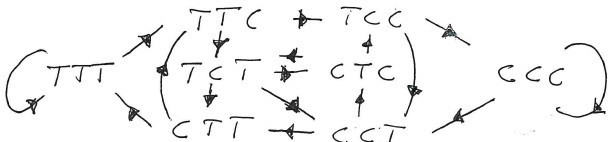
\includegraphics[scale=1]{Scam della moneta}
\end{center} 
Facciamo un esempio per spiegare questo concetto controintuitivo: \\
Supponiamo il caso più facile (perchè più favorevole per il banco), ovvero il caso in cui il giocatore scelga la terna $CCC$ (o equivalentemente $TTT$). Allora guardando il grafo o la tabella sottostante sappiamo che il banco sceglierà la terna $TCC$. Perchè questa terna è così vantaggiosa e gli da una probabilità di vincere così alta? \\
La motivazione sta nel fatto che l'unica speranza che il primo giocatore ha di vincere è che esca croce per tre volte consecutive al primo tentativo. Infatti, se uscisse testa anche solo una volta, il povero giocatore non avrebbe speranza di vittoria, perchè a questo punto se anche uscisse croce per tre volte di fila, la prima terna vincente a uscire sarebbe quella del banco, che gli garantirebbe quindi la vittoria. \\
\begin{center}
	\begin{tabular}{ |p{3.4cm}|p{3.7cm}|p{5cm}| }
		\hline
		\textbf{Primo giocatore} & \textbf{Secondo giocatore} & \textbf{Probabilità di vincita del primo giocatore} \\
 		\hline
 		\ \ \ \ \ \ \ \ \ $\underline{CC}C$ & \ \ \ \ \ \ \ \ \ \ $T\underline{CC}$ & \ \ \ \ \ \ \ \ \ \ \ \ \ \ $7$ a $1$ \\
 		\hline
 		\ \ \ \ \ \ \ \ \ $\underline{CC}T$ & \ \ \ \ \ \ \ \ \ \ $T\underline{CC}$ & \ \ \ \ \ \ \ \ \ \ \ \ \ \ $3$ a $1$ \\
 		\hline
 		\ \ \ \ \ \ \ \ \ $\underline{CT}C$ & \ \ \ \ \ \ \ \ \ \ $C\underline{CT}$ & \ \ \ \ \ \ \ \ \ \ \ \ \ \ $2$ a $1$ \\
 		\hline
 		\ \ \ \ \ \ \ \ \ $\underline{CT}T$ & \ \ \ \ \ \ \ \ \ \ $C\underline{CT}$ & \ \ \ \ \ \ \ \ \ \ \ \ \ \ $2$ a $1$ \\
 		\hline
 		\ \ \ \ \ \ \ \ \ $\underline{TC}C$ & \ \ \ \ \ \ \ \ \ \ $T\underline{TC}$ & \ \ \ \ \ \ \ \ \ \ \ \ \ \ $2$ a $1$ \\
 		\hline
 		\ \ \ \ \ \ \ \ \ $\underline{TC}T$ & \ \ \ \ \ \ \ \ \ \ $T\underline{TC}$ & \ \ \ \ \ \ \ \ \ \ \ \ \ \ $2$ a $1$ \\
 		\hline  
 		\ \ \ \ \ \ \ \ \ $\underline{TT}C$ & \ \ \ \ \ \ \ \ \ \ $C\underline{TT}$ & \ \ \ \ \ \ \ \ \ \ \ \ \ \ $3$ a $1$ \\
 		\hline
 		\ \ \ \ \ \ \ \ \ $\underline{TT}T$ & \ \ \ \ \ \ \ \ \ \ $C\underline{TT}$ & \ \ \ \ \ \ \ \ \ \ \ \ \ \ $7$ a $1$ \\
 		\hline
	\end{tabular} 
\end{center}
\subsection{Random walk non omogeneo}
Abbiamo una linea retta discretizzata con passo spaziale $\Delta x$ e passo temporale $\Delta t$. Supponiamo che, a differenza del random walk classico, la particella oltre a poter fare un passo nelle due direzioni possa farne due contemporaneamente (quindi un salto di lunghezza doppia) e come al solito supponiamo che tale particella non possa stare ferma. Supponiamo inoltre che sia leggermente più probabile fare un salto doppio piuttosto che farne uno singolo. Per cui abbiamo quattro probabilità:
$$
	P_{++} = P_{--} = \frac{1}{4}(1+\epsilon x) \ \ \ x \ \longrightarrow \ x \pm 2\Delta x
$$
$$
	P_+ = P_- = \frac{1}{4}(1-\epsilon x) \ \ \ x \ \longrightarrow \ x \pm \Delta x
$$
dove, come atteso, notiamo che la somma delle quattro probabilità fa 1.\\
Osservando queste probabilità notiamo che queste sono interpretabili come l'effetto di un gradiente di temperatura, perchè la particella ha una probabilità più alta di fare un salto doppio quando si trova nella regione delle $x$ positive, mentre ha più probabilità di fare salti singoli quando si trova nella regione delle $x$ negative. Questo quindi è interpretabile dicendo che nella regione $x>0$ la particella ha energia cinetica maggiore rispetto alla regione $x<0$, e dalla termodinamica sappiamo che questo si traduce in una temperatura maggiore in questa regione. 
Diciamo quindi che la parte delle $x$ negative è la zona fredda, mentre quella delle $x$ positive è la zona calda. \\
La media degli spostamenti è uguale a 0, mentre la varianza è:
$$
	\lang \Delta x^2 \rang = (4\Delta x^2)(P_{++} + P_{--}) + \Delta x^2(P_+ + P_-) = \left(\frac{5}{2} + \frac{3}{2}\epsilon x\right)\Delta x^2
$$
e chiaramente questa varianza non è costante. \\
Ora ci chiediamo, supponendo di far partire le particelle dall'origine, queste andranno di più a destra o a sinistra? \\
In un processo fisico le fluttuazioni sono causate da gradi di libertà nascosti. \\ \\ \\
Passiamo al limite continuo, ovvero mandiamo i passi temporali e spaziali a 0, ma manteniamo costante il rapporto $\Delta x/\Delta t$. Otteniamo la seguente equazione:
$$
	\frac{\partial p}{\partial t} = \frac{1}{2}\frac{\partial^2}{\partial x^2}T(x)p
$$
dove $p(x,t)$ è la distribuzione di probabilità. \\
A questo punto calcoliamo quindi il valor medio di x:
$$
	\lang x \rang = \int xp(x,t)dx
$$ \\ \\
Se invece $\Delta T$ non è trascurabile:
$$
	\frac{\partial p}{\partial t} = \frac{1}{2}\frac{\partial}{\partial x}T(x)\frac{\partial}{\partial x}p
$$
Porco dio non si è capito un cazzo!
\subsection{Dinamica di un neurone o del battito cardiaco}
Un neurone può creare un potenziale di propagazione. Quando viene generato il potenziale questo ha una crescita molto rapida, per poi decrescere e stabilizzarsi attorno allo 0. \\
Indichiamo con $x$ la dimensione della cellula e con $b$ la corrente che passa in essa, e le variazioni di queste grandezze sono:
$$
	\epsilon\frac{dx}{dt} = -(x^3 - Tx + b)
$$
$$
	\frac{db}{dt} = x - x_0
$$
Il sistema è in equilibrio per: $x = x_0$, \ $b_0 = -x_0^3 + Tx_0$ \\ \\ \\ \\
Studiamo la stabilità dell'equilibrio:
$$
	\epsilon \frac{d}{dt}\Delta x = -(3x_0^2-T)\Delta x - \Delta b
$$
$$
	\frac{d}{dt}\Delta b = \Delta x
$$	
Abbiamo la matrice:
$$
	\begin{pmatrix}
	-\dfrac{3x_0^2 + T}{\epsilon} & -\dfrac{1}{\epsilon} \\
	1 & 0
	\end{pmatrix}
$$
Vogliamo studiare gli autovalori e autovettori di questa matrice. Notiamo che il determinante è positivo, quindi perchè gli autovalori siano negativi la traccia dere essere negativa, quindi dobbiamo limitarci a studiare:
$$
	-3x_0^2 + T < 0
$$ \\ \\ \\
Possiamo ora accoppiare due neuroni:
$$
	\epsilon\frac{dx}{dt} = -(x^3 - Tx + b) \ \ \ \ \ \ \ \epsilon\frac{dy}{dt} = -(y^3 - Ty + b')
$$
$$
	\frac{db}{dt} = x - y \ \ \ \ \ \ \ \ \ \ \ \ \ \frac{db'}{dt} = y - x
$$
dove abbiamo le condizioni al contorno $x(0) = x_0$ e $y(0) = x_1$. \\ \\ \\ 


\subsection{Modello di Fitzhugh-Maguno}
Maguno capì che il modello fisiologico poteva essere ricondotto al modello di wababu, quindi per studiare i segnali prodotti dal neurone si può usare questo modello, che è molto più semplice di quello fisiologico. Le equazioni del modello sono le seguenti:
$$
	\frac{dx}{dx} = x - \frac{x^3}{3} - w + I
$$
$$
	\frac{dw}{dt} = \frac{1}{\tau} (x+a-bw)
$$
dove $x$ è il potenziale di membrana e $w$ è la corrente. Il parametro $1/\tau$ è molto piccolo. Il termine $b$ è un termine dissipativo che dice che la corrente tende a smorzarsi. $I$ è lo stimolo esterno. \\ \\
Come prima si ottiene una cubica, che dipende dallo stimolo $I$, che ha la funzione di alzare o abbassare la curva (incide sul punto di intersezione con l'asse delle ordinate). 
$$
	w = x - \frac{x^3}{3} + I
$$
Si ha anche una retta data da:
$$
	w = \frac{x+a}{b}
$$ 
questa retta può intersecare la cubica in uno o più punti. Se sto sopra la curva, la x tende ad andare verso sinistra, mentre se sono sotto, la x tende ad andare verso destra.
Ora vogliamo studiare se il punto $p$, ovvero l'intersezione tra la retta e la cubica, è stabile. 
$$
	\frac{x+a}{b} = x - \frac{x^3}{3} + I \ \ \longrightarrow \ \ \begin{cases}
	\delta \dot{x} = (1-x_p^2)\delta x - \delta w \\
	\delta \dot{w} = \frac{1}{\tau} (\delta x - b \delta w)
	\end{cases}
$$
Si ottiene quindi la matrice:
$$
	\begin{pmatrix}
		(1-x_p^2) & -1 \\
		\dfrac{1}{\tau} & -\dfrac{b}{\tau}
	\end{pmatrix}
$$
Questa matrice ha determinante:
$$
	det \ A = -\frac{b}{\tau}(1-x_p^2) + \frac{1}{\tau}
$$
e notiamo che se $|x_p|$ è grande si ha stabilità.


\end{document}